%!TEX root = ../main.tex
\newcommand{\vcenteredinclude}[1]{\begingroup
\setbox0=\hbox{\includegraphics[width = 0.3\textwidth]{#1}}%
\parbox{\wd0}{\box0}\endgroup}

\begin{frame}{Algorithmes évolutionnistes}
   \textbf{Algorithmes évolutionnistes (AE)}\\
  \textit{Type : }Métaheuristique\\
  \textit{Stochastique : } Oui\\
  \textit{Caractéristique : } Évolution d'une population de solutions
  \vspace{0.5cm}
  \hrule
\vspace{0.2cm}
\textbf{Principes}\\
1. Chaque solution possède un niveau \textit{d'adaptation} \\
2. Opérateurs de \textit{variation} pour générer de nouvelles solutions  \\
3. Opérateurs de \textit{sélection} pour améliorer l'adaptation des solutions
\end{frame}

\begin{frame}{Schéma d'un AE}
	\begin{figure}[tb]
    	\centering
    	\includegraphics<1>[width=0.95\textwidth]{figures/cycle_evolution1.pdf}
      \includegraphics<2>[width=0.95\textwidth]{figures/cycle_evolution2.pdf}
	\end{figure} 
\end{frame}


% \begin{frame}{Caractéristiques des AE}
	
% \begin{figure}[tb]
%     \centering
%     \includegraphics<1>[width=0.95\textwidth]{figures/triforce.pdf}
% \end{figure} 
% \end{frame}

\begin{frame}{Problème du sac à dos}
\vspace{-10pt}
\textbf{Knapsack problem}\\
Un revendeur de chocolat doit distribuer sa précieuse cargaison et récolter ses gains. Malheureusement, il n'a le temps de faire qu'une seule tournée avant que son fournisseur n'arrive. De plus, son sac à dos peut transporter au plus une masse $M$. \\
\textit{Quel est le sous-ensemble de boîtes lui permettant de garder ses deux jambes?}
  
\begin{figure}[tb]
    \centering
    \includegraphics<1>[width=0.85\textwidth]{figures/knapsack.pdf}
\end{figure} 
\end{frame}

\begin{frame}{Implémentation d'un algorithme génétique}
   \vspace{-15pt}
   \textbf{Représentation du génome }  \\
   \begin{figure}[h]
   \centering
   \includegraphics<1>[width=0.35\textwidth]{figures/bitString.pdf} 
   \end{figure}
   \vspace{-5pt}
   \textbf{Niveau d'adaptation} \\
   L'adaptation $x_i$ d'un individu $i$ correspond à la valeur totale des objets sélectionnés. \\ \vspace{15pt}
   \textbf{Sélection des parents } \\ 
   Soient des individus $i,j$ choisis aléatoirement. On sélectionne $i$ si 
   \begin{align*}
   x_i \geq x_j
   \end{align*}
\end{frame}

\begin{frame}{Implémentation d'un algorithme génétique}

   \textbf{Croisement des parents } \\ \vspace{5pt}
  \begin{figure}[h]
   \centering
   \includegraphics<1>[width=0.9\textwidth]{figures/croisement.pdf} 
   \end{figure} 
   \textbf{Mutation } \\ \vspace{5pt}
  \begin{figure}[h]
   \centering
   \includegraphics<1>[width=0.9\textwidth]{figures/mutation.pdf} 
   \end{figure}
   \textit{Élitisme }

\end{frame}


\begin{frame}{Problème du sac à dos - Évolution du génome}
\textbf{Occurence des gènes à l'intérieur de la population}
  \begin{figure}[h!]
    \centering
    \href{run:figures/genome_dist.mp4}{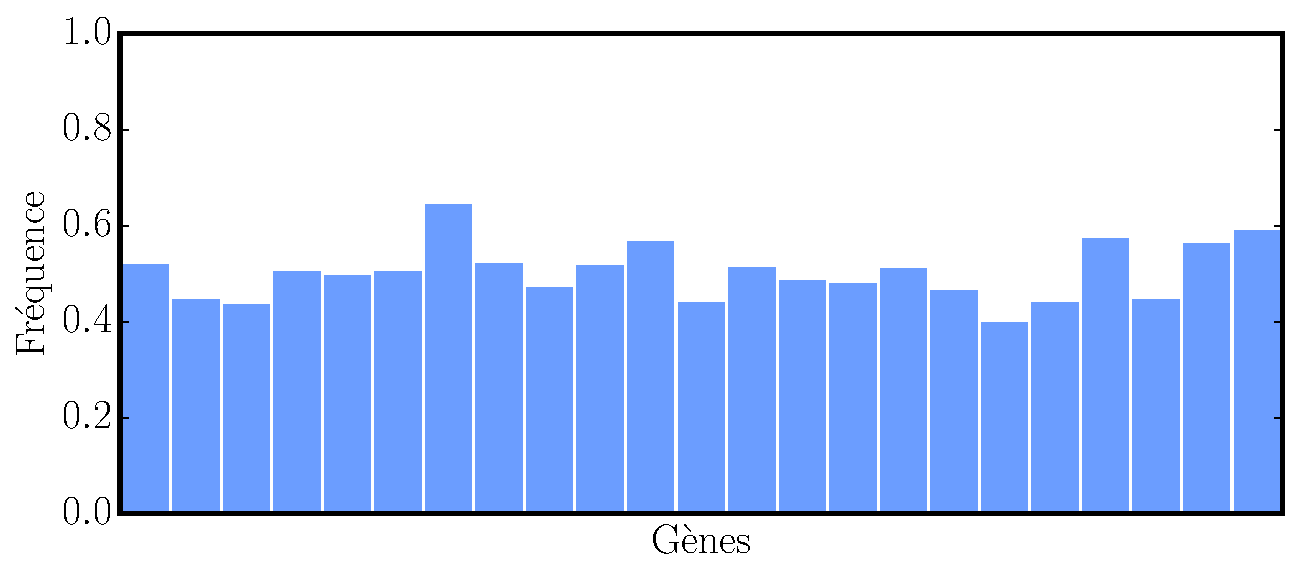
\includegraphics[width=0.95\textwidth]{figures/genome_dist.pdf}}
  \end{figure}
  \vspace{-30pt}
  \begin{figure}[h!]
    \centering
    \hspace{25pt}
\includegraphics[width=0.85\textwidth]{figures/formes.pdf}
  \end{figure}
\end{frame}

\begin{frame}{Problème du sac à dos - Adaptation}
\vspace{-10pt}
\textbf{Niveau d'adaptation des populations}
  \begin{figure}[h!]
    \centering
    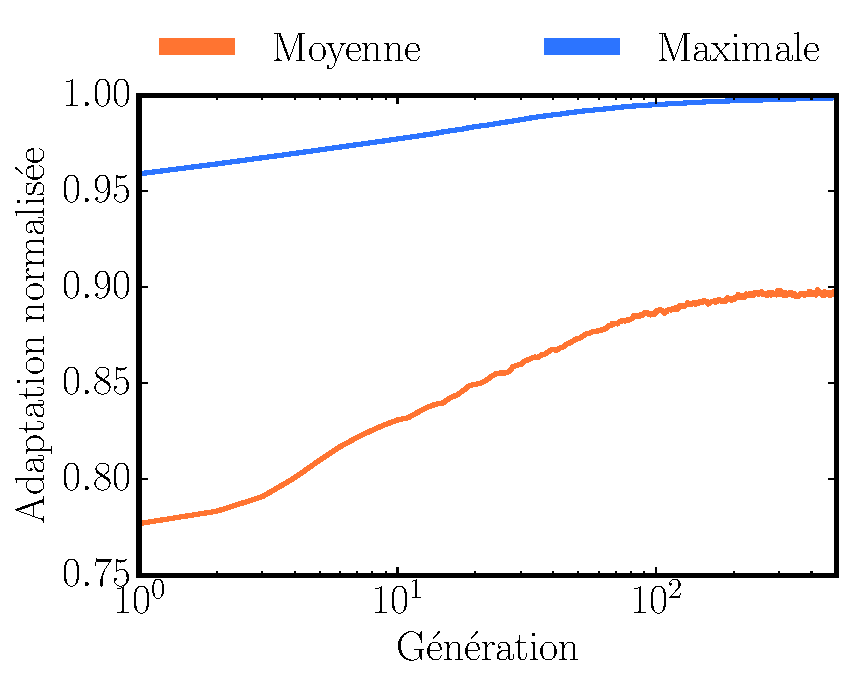
\includegraphics[width=0.75\textwidth]{figures/knapsack_adaptation.pdf}
  \end{figure}
\end{frame}